\capitulo{5}{Aspectos relevantes del desarrollo del proyecto}


\section{Descripción del juego}

\subsection{Introducción}
Para entender todo el proceso de entrenamiento del bot inteligente que voy a implementar considero necesario entender el funcionamiento y reglas del juego así como ciertas particularidades relacionadas con la captura y uso de datos.
\subsection{Diseño de reglas y desarrollo del juego}

El juego va a ser un «mata-marcianos» de tipo arcade, un juego infinito en el que el jugador aspira a alcanzar la máxima puntuación de forma individual. Este tipo de juegos era típico de los salones recreativos y centros comerciales en la década de los años ochenta. En este caso nos ponemos a los mandos de una nave espacial que ha de evitar que los enemigos invasores traspasen la zona inferior de la pantalla (nuestro territorio). Los enemigos aparecen en oleadas y se limitan a avanzar oscilando hacia su objetivo. El jugador ha de eliminar el máximo número de enemigos posibles sin impactar contra ellos. Cuanto menos se acerquen a la zona inferior de la pantalla mayor será la puntuación que otorgue su eliminación. Si los enemigos llegan a nuestro territorio restarán una cantidad fija de puntos, por lo que nuestra puntuación final se verá notablemente mermada.



En el apartado gráfico se optó por un aire retro, algo que recordase a las primeras máquinas arcade o consolas de videojuegos. En primer lugar me decanté por imitar el estilo de la \emph{Game Boy}, consola que triunfó en los 90. Para ello se seleccionó una paleta de colores que recordase a los gráficos de la época. Para el jugador y los enemigos se utilizó un pack de Sprites gratuito de la tienda de Unity3D\footnote{Estos Sprites solo se utilizaron en la versión inicial, más adelante son sustituidos por unos nuevos hechos por mí.}.

\begin{figure}[]
\centering

\includegraphics[width=0.1\textwidth]{./img/paleta_de_colores}
\caption{Paleta de colores}
\end{figure}

\begin{figure}[]
\centering
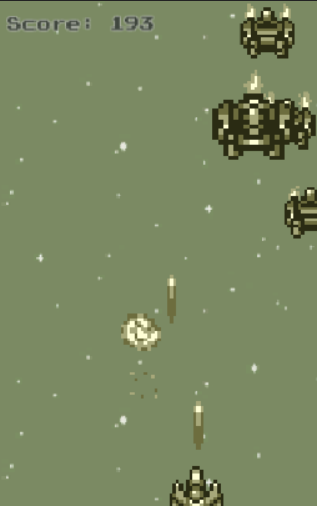
\includegraphics[width=0.5\textwidth]{./img/ifaz_v1}
\caption{Interfaz. Versión 1}
\end{figure}

\subsection{Evolución de las reglas del juego}

Ya tenía la primera versión lista para jugar. En este punto se decidió establecer unas reglas un poco más «especiales» para simplificar el proceso. En primer lugar, los enemigos no atacan al jugador con ningún tipo de proyectil, se limitan a avanzar oscilando a una velocidad constante. Por otro lado, se limitará el número de enemigos visibles simultáneamente en la pantalla con el fin de poder hacen una instancia de tamaño constante y no perder enemigos en la captura de datos. Para darle un poco de dinamismo y evitar que el jugador deje pulsada la tecla de disparo infinitamente, se ha implementado un sistema de calentamiento del arma. Este sistema hace que los disparos consecutivos calienten el arma y si no se dispara, se enfríe lentamente. Si el arma llega al máximo de temperatura dejará de disparar. El sistema de calentamiento del arma dio lugar a la idea de implementar unos «power-up» o potenciadores. Estos serán de dos tipos, uno enfría de golpe el arma una determinada cantidad y otro duplica en número de balas disparadas simultáneamente. Esto, como se describirá más adelante, condicionará la estructura de las instancias.

Como última aclaración, los «sujetos de prueba», a los que el agente inteligente deberá imitar, se aburrían jugándolo, por lo que se introdujo un jefe que tendría una enorme cantidad de vida. Este jefe aparecerá una vez por minuto jugado y restará muchos más puntos que los enemigos estándar. La eliminación de este tipo de enemigo conlleva un gran calentamiento del arma y, por tanto, un estrés añadido al jugador, que tendrá que estar listo en todo momento para este tipo de combate.

\subsection{Evolución del interfaz gráfica}
La primera versión de la interfaz del juego tenía una \emph{aspect ratio}  de 5:3, lo que no le hacía agradable a la vista, ni dejaba espacio para otros elementos de la interfaz. Por este motivo, se decidió revisar el diseño inicial.

Se diseñó un menú principal que dejaba elegir entre empezar a jugar o salir del juego. Esta pantalla fue diseñada por el ilustrador Luis G. Contreras\footnote{http://www.borratajo.es/}. Para la interfaz del juego se amplió la paleta de colores, dejando de lado el aspecto \emph{Game Boy} pero manteniendo un aire retro.


\begin{figure}[]
\centering
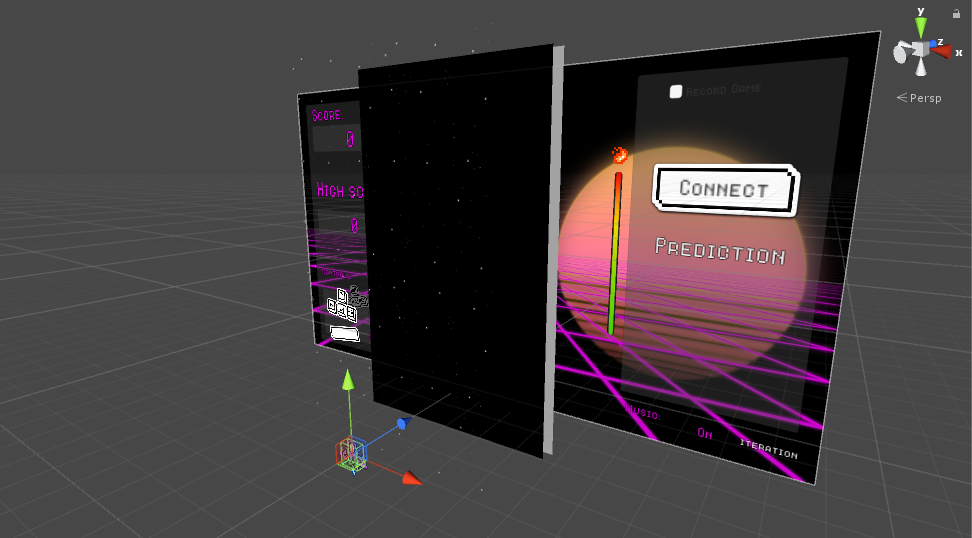
\includegraphics[width=0.8\textwidth]{./img/UnityIfaz}
\caption{Interfaz de desarrollo Unity3D}
\end{figure}


\begin{figure}[]
\centering
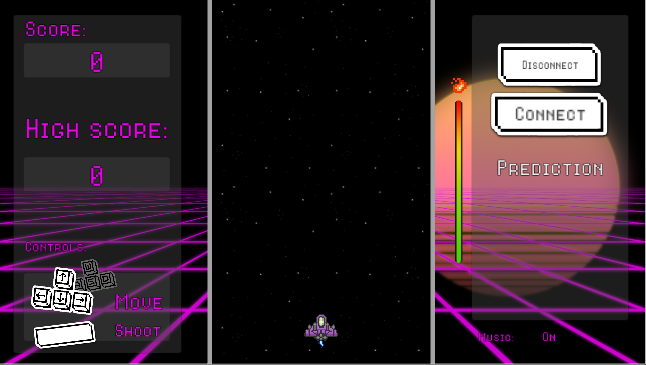
\includegraphics[width=0.8\textwidth]{./img/ifaz_v2}
\caption{Evolución de diseño de la interfaz}
\end{figure}

\section{Comunicación entre Scripts}

\subsection{introducción}
Para el desarrollo del proyecto, se han utilizado dos lenguajes de programación. Por un lado c\#, que ha sido uno de los lenguajes más utilizado para el desarrollo de videojuegos en la historia reciente, por otro, Python, que es el lenguaje en el que están las bibliotecas utilizadas para el entrenamiento de nuestro sistema inteligente. Por este motivo, era necesario encontrar la forma de que el juego pudiera ejecutar los scripts de Python, además de pasarle la correspondiente información. El proceso de comunicación ha sido uno de los puntos que más problemas me ha dado a lo largo del desarrollo del proyecto, ya que hubo que probar varias alternativas hasta dar con la correcta.

\subsection{Pythonet}
En primer lugar estudié la posibilidad de integrar Python en c\#, de tal forma que pudiese ejecutar pequeños scripts de Python dentro de mi código en c\#. Para esta integración se probé a utilizar Pythonet. Pythonet, como pone en su pagina web\footnote{https://github.com/Pythonnet/Pythonnet}, permitiría a Python interactuar con el CLR\footnote{CLR: ( Common Language Runtime) Máquina virtual de .net que controla la ejecución del le srcipts .net} de .net e incrustar código Python en .net. Tras númerosas pruebas no hubo forma de ejecutar una sola línea de Python desde un script Monobehaviour. MonoBehaviour es la clase maestra de la que heredan todos los scripts de unity. Esta clase proporciona las fuciones necesarias para la ejecución del juego. Las funciones elementales son Start() y Update(), pero disponemos de muchas más. 


\subsection{IronPython}
La siguiente herramienta con la que se estuvo trabajando fue \emph{IronPython}. \emph{IronPython} prometía unas utilidades muy similares a Pythonet, o incluso mejores, pero tras varias horas de lectura de la documentación encuentro algo que tira por tierra mis expectativas, \emph{IronPython} aún no es compatible al cien por cien con Scikit-learn.

\subsection{Pipes o tuberías}
Comienza una nuevas vía de investigación, era el turno de los pipes (o tuberías) de Python. En internet no había demasiada información y la poca que había no era muy clara, pero aún así me puse manos a la obra y a las pocas horas ya tenía dos scripts de Python comunicándose entre ellos. Bien, ahora solo quedaba que se comunicase con mi aplicación en .net. Este ultimo paso no hubo forma de llevarlo a cabo, no conseguí que ambas aplicaciones intercambiasen mensajes de forma correcta.

\subsection{Sockets}
Finalmente, me decanté por utilizar, o bien WebServices, o bien sockets. Como la opción de los sockets me parecía en principio más sencilla me puse manos a la obra. Primero hice un servidor de sockets y un cliente en Python, y funcionó. El script era sencillo, un simple eco, cuando alguien se conectaba enviaba de vuelta toda la información que recibiese. El siguiente paso lógico era hacer lo propio en .net, y funcionó, ya tenía las aplicaciones intercambiando mensajes.

El funcionamiento final consiste en un script de Python que al ejecutarse abre un socket anónimo que se queda a la espera de una conexión, cuando alguien se conecta empieza a escuchar y procesar todos los mensajes que le llegan pasándoselos al modelo del sistema inteligente, una vez procesados, por la misma vía responde con el resultado calculado.


\section{Definiendo las instancias}\label{sec:instancias}

Para dotar a la máquina de la capacidad de aprender es necesario, como en el aprendizaje de los seres humanos, una serie de estímulos. Estos estímulos, en mi caso, se traducen en una serie de estados o instancias. Para todas la pruebas iniciales se empezó utilizando un clasificador Random forest\footnote{Al poco tiempo se descartó la validación cruzada ya que en la teoría rozaba el 97\% de acierto y en la práctica se alejaba mucho de la realidad y , por lo tanto, no nos sirve para validar con qué eficacia imita al humano}.

Para empezar, se comenzó seleccionando los que parecían más relevantes, como la posición absoluta del jugador y la posición absoluta de los enemigos  en el campo de batalla. Solo formaba parte de la clase la última tecla pulsada por el usuario, que podía ser Arriba, Abajo, Izquierda, Derecha, Disparo o No disparo. Para entrenar un agente en número de atributos de entrada debe ser inmutable, por lo que se estableció un máximo de cuatro enemigos en pantalla de forma simultánea. Dado que yo estaba programando el videojuego yo tenía el control absoluto de todas las variables.


\begin{table}[]
    \centering
    \begin{tabular}{c}
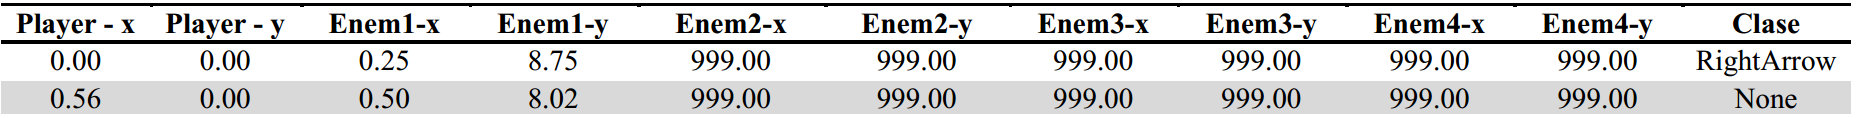
\includegraphics[width=\textwidth]{../img/tabla1-estados1}
    \end{tabular}
    \caption{Primera versión Instancia}
    \label{tab:Primera_versión}
\end{table}

Tras un primer entrenamiento, con un número no muy alto de instancias (~4000) los resultados no eran muy satisfactorios. En siguiente iteración se observó que había otro parámetro más que nos podría ayudar a tomar decisiones, la vida del enemigo.



\begin{table}[]
    \centering
    \begin{tabular}{c}
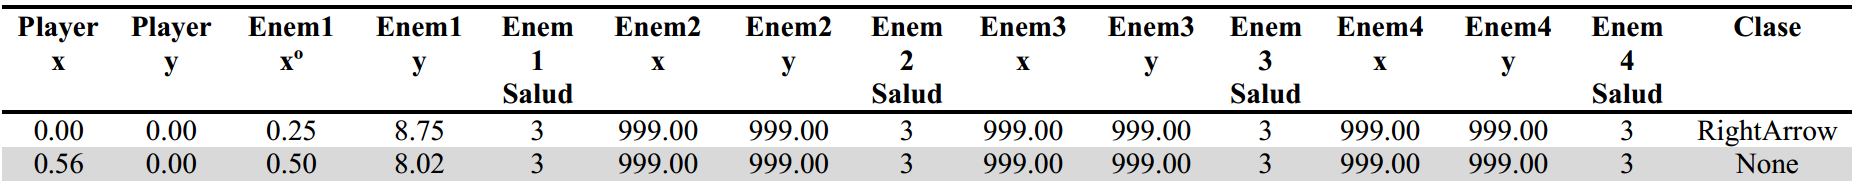
\includegraphics[width=\textwidth]{../img/tabla2-estados2}
    \end{tabular}
    \caption{Segunda versión Instancia}
    \label{tab:Segunda_versión}
\end{table}


De forma paralela se iban realizado tests de jugabilidad con diferentes usuarios, dado que el arma se calentaba rápidamente, se optó por introducir en el juego los «power-up». Llegados a este punto se decidió seguir aumentando el número de atributos con el fin de extraer toda la información que podría tener un humano de la partida. Así que ahora la instancia tendrá también la posición absoluta de los «power-up». 

\begin{table}[]
    \centering
    \begin{tabular}{c}
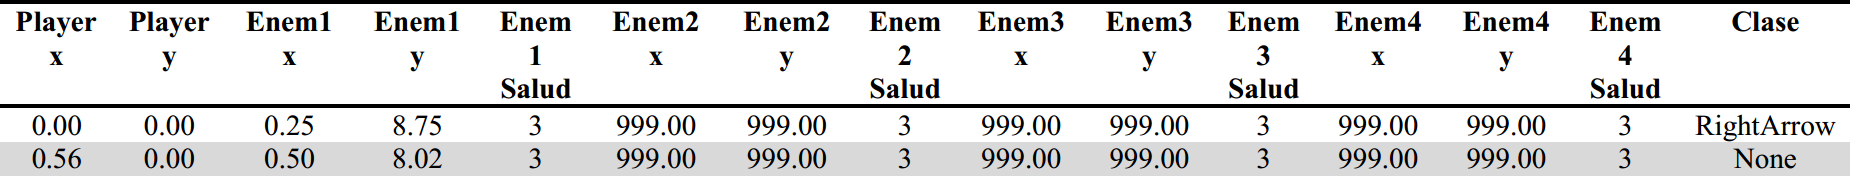
\includegraphics[width=\textwidth]{../img/tabla3-estados3}
    \end{tabular}
    \caption{Tercera versión Instancia}
    \label{tab:Tercera_versión}
\end{table}
    


La posición de los enemigos, como se puede ver en las ilustraciones adjuntas, venían dados por posiciónX, posicionY y vida restante. Para facilitar al modelo la clasificación lo que hago el crear un «heat-map» con las posiciones de los enemigos en una matriz. Este heat-map o mapa de densidad proporciona la información de la cantidad de enemigos que hay en un un sector concreto. Pudiendo establecer el tamaño... 

\begin{figure}[]
  \centering
  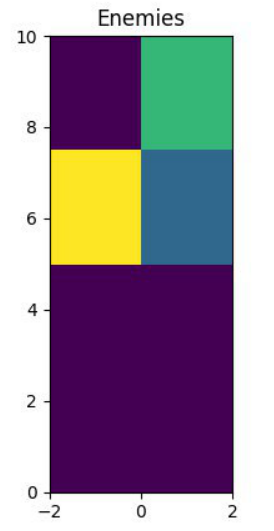
\includegraphics[width=0.35\textwidth]{../img/enemies_heat_map}\label{fig:f1}
  \hfill
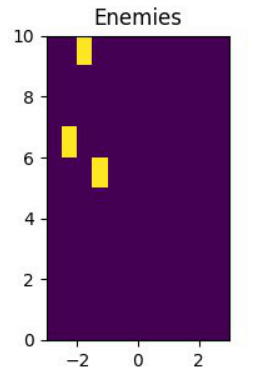
\includegraphics[width=0.43\textwidth]{../img/enemies_heat_map_1}\label{fig:f2}
  \caption{Heat-maps con diferentes garnularidades}
\end{figure}



Ya tenía definidas las instancias con las que empezarían mis primeros entrenamientos. Esta vez comencé con un dataset con menos de 1000 entradas y los resultados seguía siendo muy mejorables, la aletoreidad de los movimientos era evidente. ¿Qué parámetros estaba teniendo yo en cuenta que no le estaba transmitiendo la instancia? La respuesta es «el tiempo». Yo, cuando jugaba, era consciente de varios atributos que no eran plasmables en una «Fotografía», que es lo que venía siendo la instancia hasta ahora. Así que para esto se seleccionaron grupos de $n$ instancias consecutivas y se concatenaron para formar una nueva instancia $n$ veces la inicial. Los atributos de mi nueva instancia serían ahora:

[instanciaT-$n$...instanciaT-2 instanciaT-1 instanciaActual][clases actuales]

En esta primera concatenación los resultados mejoraron notablemente. El juego se movía por fin de una forma aceptable. Aún así, se decidió incluir en la instancia los movimientos realizados en las acciones anteriores, ya que se pensó que podría ser que también fuesen relevantes. 

Se realizaron entrenamientos de prueba con varios dataSet y se observó un problema común en todas la iteraciones. Cuando se acercaba a los bordes de la zona de juego, dejaba de responder correctamente, realizando movimientos aleatorios, llegando incluso a dejar de actuar totalmente. El problema residía en la forma de jugar del los usuarios.

\imagenflotante{posJugA}{Posiciones del jugador}\label{fig:pos_jugador}

Los jugadores humanos tienden, como es lógico, a jugar en el centro de la pantalla, por lo que en el centro de la pantalla se tienen muchas instancias de las que aprender en esa zona, pero en los bordes, las instancias eran casi nulas. La figura \ref{fig:pos_jugador} representa la cantidad de muestras (instancias) en relación a la posición absoluta del jugador en el terreno de juego.

En este punto hay un cambio radical en la estructura de las instancias. Ya que una posición absoluta del jugador y los enemigos da lugar a estados únicos muy amplios. Decidí que una buena forma de reducir esta gran cantidad de estados únicos era trabajar con la distancia relativa del jugador a los diferentes enemigos. 


\begin{table}[]
\centering
\begin{tabular}{c|c|c|}
\hline
\rowcolor[HTML]{C0C0C0} 
\multicolumn{1}{|c|}{\cellcolor[HTML]{C0C0C0}Tipo}                                           & Atributos                                                                                             & Total \\ \hline
\multicolumn{1}{|c|}{\begin{tabular}[c]{@{}c@{}}Información \\     del jugador\end{tabular}} & \begin{tabular}[c]{@{}c@{}}PosisiónX,\\      PosiciónY,\\      Temperatura del arma\end{tabular}      & 3     \\ \hline
\multicolumn{1}{|c|}{\begin{tabular}[c]{@{}c@{}}Información \\     del enemigo\end{tabular}} & \begin{tabular}[c]{@{}c@{}}PosX 1-6\\     PosY 1-6\\     Vida restante 1-6\end{tabular}               & 18    \\ \hline
\multicolumn{1}{|c|}{\begin{tabular}[c]{@{}c@{}}Información\\ Power-Up\end{tabular}}         & \begin{tabular}[c]{@{}c@{}}Power-Up1 PosX\\ Power-Up1 PosY\\ Power-Up2 PosX\\ Power-Up2 PosY\end{tabular} & 4     \\ \hline
\multicolumn{1}{|c|}{\begin{tabular}[c]{@{}c@{}}Otra\\   información\end{tabular}}           & \begin{tabular}[c]{@{}c@{}}TimeStamp\\     Score\end{tabular}                                         & 2     \\ \hline
\multicolumn{1}{|c|}{Clases}                                                                 & \begin{tabular}[c]{@{}c@{}}Arriba-Abajo\\     Izquierda-Derecha\\     Dispara-NoDispara\end{tabular}  & 3     \\ \hline
                                                                                             & Total                                                                                                 & 30    \\ \cline{2-3} 
\end{tabular}
\caption{Cuarta versión Instancia}
\label{my-label}
\end{table}


\section{«visión» del bot}

La representación por la que me decanté finalmente fue la que almacenaba la distancia relativa a los diferentes enemigos. Para obtener una cantidad de atributos constante, lo que se hizo fue definir una serie de rayos procedentes del jugador como se ve en la ilustración \ref{fig:playerView}.


\imagenflotante{playerView}{Visión del Bot}

Para obtener la información, se irán haciendo barridos cada 0.25 segundos. Si el rayo impacta contra un enemigo se almacenará la distancia en línea recta al mismo. Si el rayo no impacta contra nada, se insertará un valor numérico especial para indicar la ausencia de información. Ésta última aproximación tiene la ventaja de que nos va a ser indiferente la cantidad de enemigos en pantalla, ya que lo que almaceno el la presencia o no de los mismos en mi campo visual. Por otro lado tiene el inconveniente de que un enemigo me puede ocultar la presencia de otro que se encuentre detrás y que, hasta que este primero no sea destruido, no nos va a ser posible conocer más información.

Finalmente tenemos una instancia con mucha información, de la cual podemos seleccionar qué atributos vamos a utilizar y cuales no.

\begin{table}[]
\centering
\begin{tabular}{c|c|c|}
\hline
\rowcolor[HTML]{C0C0C0} 
\multicolumn{1}{|c|}{\cellcolor[HTML]{C0C0C0}Tipo}                                           & Atributos                                                                                                      & Total                   \\ \hline
\multicolumn{1}{|c|}{\begin{tabular}[c]{@{}c@{}}Información \\     del jugador\end{tabular}} & \begin{tabular}[c]{@{}c@{}}PosisiónX,\\      PosiciónY,\\      Temperatura del arma\end{tabular}               & 3                       \\ \hline
\multicolumn{1}{|c|}{\begin{tabular}[c]{@{}c@{}}Información \\     del enemigo\end{tabular}} & \begin{tabular}[c]{@{}c@{}}PosX\\   1-6\\     PosY 1-6\\     Vida restante 1-6\\     Raycast 1-27\end{tabular} & 45                      \\ \hline
\multicolumn{1}{|c|}{\begin{tabular}[c]{@{}c@{}}Otra\\   información\end{tabular}}           & \begin{tabular}[c]{@{}c@{}}TimeStamp\\     Score\end{tabular}                                                  & 2                       \\ \hline
\multicolumn{1}{|c|}{Clases}                                                                 & \begin{tabular}[c]{@{}c@{}}Arriba-Abajo\\     Izquierda-Derecha\\     Dispara-NoDispara\end{tabular}           & 3                       \\ \hline
\multicolumn{1}{l|}{}                                                                        & \multicolumn{1}{l|}{Total}                                                                                     & \multicolumn{1}{l|}{53} \\ \cline{2-3} 
\end{tabular}
\caption{Quinta versión Instancia (Final)}
\label{my-label}
\end{table}


\section{Entrenamiento}
Una vez tenemos definido el tipo de instancia y el conjunto de datos con los que vamos a trabajar procedemos a entrenar el modelo del agente inteligente. Se optó por empezar entrenando un clasificador sencillo, un clasificador que nos permitiese saber hasta dónde podría llegar, ya que en un principio desconocía por completo las herramientas de aprendizaje máquina.

\section{Entrenamiento con árboles de decisión}

La primera opción barajada fueron los árboles de decisión. Este es uno de los muchos clasificadores que nos proporciona la biblioteca sicikit-learn. Se utilizaron dos tipos de clasificador, un de árbol de decisión (Decission Tree) y un Random-forest. 

 La implementación de este modelo consta de varios scripts de Python que realizarán las tareas de entrenamiento, procesado de instancias y predicción. En el apartado de entrenamiento ambos tienen una implementación idéntica, sólo vamos a cambiar la invocación al un método u otro a la hora de generar el modelo.
 
 
 Para utilizar este modelo de entrenamiento he implementado dos scripts. El primero de ellos, denominado «Trainer.py» tiene la función de generar y guardar el modelo. El segundo, «Predictor.py» , mucho mas simple, se limita a llamar a la función \emph{predict} del modelo. A pesar de ser un script muy elemental, se decidió dejarlo por separado por si era necesario un preprocesado antes de devolver el resultado, cosa que finalmente sí que ocurrió. 
 

\section{Entrenamiento con algoritmo evolutivo}

En primer lugar, nuestra idea era evolucionar un modelo entrenado para que funcionase por imitación, por este motivo se comenzó utilizando conjunto de datos utilizado en los casos anteriores para entrenar un perceptrón multicapa (MLP). 

Todo este proceso lo vamos a realizar utilizando un \emph{pipeline}. Un \emph{pipeline} nos permite realizar varios pasos para crear un modelo de forma automática. En este caso nuestro \emph{pipeline} consta de dos pasos. El primero es un \emph{Standard Scaler}, que nos va a tomar los elementos del conjunto de datos y nos los va a normalizar entre $0$ y $1$. Este paso se realiza para reducir el ruido que nos podemos encontrar, haciendo que los valores más alejados del conjunto principal tengan menos efecto en la toma de decisiones. El segundo paso es el clasificador, que va a conformar el modelo. Este clasificador, que nos proporciona la biblioteca scikit-learn, tiene unos parámetros definidos por defecto, pero podemos indicar los nuestros para conseguir que se adapte mejor a nuestro problema.

Los primeros entrenamientos se realizaron con los parámetros por defecto del MLP que nos proporciona la biblioteca sckit-learn. Los resultados de estos entrenamientos eran desastrosos por lo que se procedió a realizar un calibrado de parámetros del MLP. Para el calibrado de parámetros se utilizó una de las herramientas que nos ofrece scikit-learn. De las dos fórmulas que nos ofrece me decanté por el Randomized Parameter Optimization. Ésta herramienta lo que hace es que, dados unas posibilidade de determinados parámetros, él los va combinado y probando aleatoriamente, de manera que finalmente te indique cuál ha dado mejores resultados. No podemos tener la certeza de que esa combinación de parámetros vaya a ser la mejor, pero ahorra tiempo.

Una vez calibrados los parámetros del MLP se procede a la neuroevolución de la red. Para este proceso se utilizaron las herramientas que nos proporciona DEAP\footnote{Se habla de esta biblioteca en el apartado Técnicas y herramientas}. 


En el proceso de neuroevolución hay que preparar el entorno en el que vamos a trabajar. Como ya se introdujo en el apartado de \emph{Conceptos teóricos}, esta preparación consta de: definir el individuo, indicar el tipo de cruce y especificar los porcentajes tanto de mutación como de cruce.

Para la definición de los individuos se utiliza un array conformado por los pesos de la red neuronal del MLP. Dado que los pesos de la red neuronal no tienen estructura de array, ha sido necesario implementar una función que realice esa tarea. Ahora, cuando la red neuronal genere un individuo lo hará en forma de array pero, cuando se proceda a probar el modelo, se volverá a convertir para que pueda ser utilizado por la red neuronal.

La función de \emph{fitness} viene dada por la media de los $n$ intentos por cada partida jugada. La media de las partidas jugadas se calcula de la siguiente manera: Cada individuo juega una partida. Una partida se compone de $n$ intentos. En cada partida, el juego genera un \emph{csv} en el que se va almacenando la puntuación de cada intento. Al final de todos los intentos, la función de \emph{fitness} lee el fichero y hace la media. Esa media es el valor de \emph{fitness} que buscamos.


Hay que definir, también, una función que genere la población inicial de acuerdo a nuestras demandas. En este caso la función generará $n$ arrays con valores aleatorios acotados a nuestro gusto.


De todos los entrenamientos realizados creo que es interesante analizar los resultados del modelo finalmente entregado:



Para la primera fase del entrenamiento se generó un clasificador MLP con seis neuronas\footnote{Este número no es un número arbitrario, surge de la evaluación mediante validación cruzada de varios modelos generados con diferentes número de neuronas}. Las poblaciones se generaron con un tamaño de diez individuos de los cuales, cuatro serían idénticos al MLP generado a partir de los datos tomados. El hecho de introducir individuos no generados aleatoriamente, nos permite «forzar» a nuestros individuos a evolucionar en una  dirección, concretamente, hacia los resultado obtenidos de los jugadores humanos. Además, introducir estos individuos agiliza notablemente el aprendizaje, ya que partimos de un modelo parcialmente entrenado, lo que nos evita todo el proceso de ensayo error del principio.

Como se puede observar en la tabla \ref{result_primer_entr}, la función converge bastante rápido, esto es observable en la cuarta generación, pues a partir de esta no cambian los resultados. Los resultados, llegados a este punto eran bastante satisfactorios, la puntuación era alta, pero estaba seguro de que eso se podía mejorar.


\begin{table}[]
\centering
\begin{tabular}{|l|l|l|l|l|l|}
\hline
\rowcolor[HTML]{C0C0C0} 
gen & nevals & avg     & std         & min      & max     \\ \hline
0   & 10     & -376515 & 527862      & -1124.18 & 601929  \\ \hline
1   & 5      & 601929  & 0           & 601929   & 601929  \\ \hline
2   & 7      & 601929  & 0           & 601929   & 601929  \\ \hline
3   & 8      & 601929  & 0           & 601929   & 601929  \\ \hline
4   & 8      & 1626.53 & 2,27374E-08 & 1626.53  & 1626.53 \\ \hline
5   & 9      & 1626.53 & 2,27374E-08 & 1626.53  & 1626.53 \\ \hline
6   & 6      & 1626.53 & 2,27374E-08 & 1626.53  & 1626.53 \\ \hline
7   & 9      & 1626.53 & 2,27374E-08 & 1626.53  & 1626.53 \\ \hline
8   & 8      & 1626.53 & 2,27374E-08 & 1626.53  & 1626.53 \\ \hline
9   & 6      & 1626.53 & 2,27374E-08 & 1626.53  & 1626.53 \\ \hline
10  & 5      & 1626.53 & 2,27374E-08 & 1626.53  & 1626.53 \\ \hline
\end{tabular}
\caption{Resultados primer entrenamiento}
\label{result_primer_entr}
\end{table}



Realicé un segundo entrenamiento, esta vez, el modelo inicial sería el mejor modelo procedente del primer entrenamiento. Del mismo modo que se procedió la primera vez, diez generaciones, poblaciones de diez individuos, ect. En la tabla \ref{result_segundo_entr} vemos que ahora converge más rapido incluso que antes y, además, incrementa la puntuación media hasta casi cuatro veces la mejor obtenida en el anterior entrenamiento.

\begin{table}[]
\centering
\begin{tabular}{|l|l|l|l|l|l|}
\hline
\rowcolor[HTML]{C0C0C0} 
gen & nevals & avg     & std     & min      & max     \\ \hline
0   & 10     & 1443.61 & 2013.27 & -1181.88 & 4802.25 \\ \hline
1   & 7      & 4712.18 & 156006  & 4441.97  & 4802.25 \\ \hline
2   & 6      & 4802.25 & 0       & 4802.25  & 4802.25 \\ \hline
3   & 8      & 4802.25 & 0       & 4802.25  & 4802.25 \\ \hline
4   & 7      & 4802.25 & 0       & 4802.25  & 4802.25 \\ \hline
5   & 6      & 4802.25 & 0       & 4802.25  & 4802.25 \\ \hline
6   & 6      & 4802.25 & 0       & 4802.25  & 4802.25 \\ \hline
7   & 7      & 4802.25 & 0       & 4802.25  & 4802.25 \\ \hline
8   & 5      & 4802.25 & 0       & 4802.25  & 4802.25 \\ \hline
9   & 5      & 4802.25 & 0       & 4802.25  & 4802.25 \\ \hline
10  & 4      & 4802.25 & 0       & 4802.25  & 4802.25 \\ \hline
\end{tabular}
\caption{Resultados segundo entrenamiento}
\label{result_segundo_entr}
\end{table}


\subsection{Bot de Telegram}
Fueron muchas la pruebas que se realizaron en el apartado de algoritmos evolutivos. Estas pruebas requerían mucho tiempo y cierta supervisión, así que, por mera curiosidad, quise ver si podía programar un bot que me enviase mensajes a través de la aplicación de mensajería \emph{Telegram}. 
En teoría un bot de \emph{Telegram} debería estar sempre activo e ir almacenando las \emph{id}  de los usuarios que quieren interactuar con el. Yo no quería dedicarle demasiado tiempo a ello, ya que no era materia fundamental de este proyecto, por lo que me limité a obtener mi \emph{id} de usuario, almacenarlo y utilizar únicamente la función de «Enviar mensaje» para avisarme de determinados eventos.


\section{Mini-proyectos Unity3D}

A lo largo de la tarea de investigación, hubo que realizar pequeños proyectos en Unity con una funcionalidad muy concreta. Los proyectos tenían como finalidad probar si se podían realizar determinadas tareas en el entorno de desarrollo de Unity. El primero que se creó, fue el que sirvió como campo de pruebas para testear la conexiones entre los scripts de Unity y los scripts de \emph{Python}. Por otro lado, tuve que hacer otro mini-proyecto para probar cómo podía lanzar mi juego desde la terminal y qué capacidad tenía para pasarle parámetros al mismo. Este último surgió a raíz de la necesidad de lanzar el juego desde \emph{Python}, ya que el algoritmo evolutivo tenía que tener la capacidad de lanzar el juego para calcular el \enpg{fitness} del individuo.